% TODO: You really need to sit down and wrap your head around all of this and how it's derived.

\subsection{Water Flow in Unsaturated Porous Media}\label{sec:richards}

The vadose zone or unsaturated zone is a region of soil between the top of the ground surface and the water table.
In the vadose zone there are two fluid phases, one gas and the other liquid (usually air and water) inside the porous soil matrix giving a three phase system; only one fluid phase (gas or liquid) exist in the saturated zone.
As a result, the transport properties in the vadose zone differ from that in a zone saturated where there are only two phases present - water and soil.\par

% TODO: This section needs serious work to make sure the nomenclature is consistently defined and referred to.
\subsubsection{Soil-Water Potential and Retention Curve}

The driving force, or soil-water potential, for the filling and draining of pore water in soils are due to a pressure and a gravitational potential and given by $\phi$.
This phenomena is called \textit{capillary potential} or \textit{matrix potential}, $\psi$, which depends on the volumetric water content $\theta$ in the soil.\par

Over the years, there has been a few attempts of characterizing the relationship between soil moisture content $\theta$ and soil water potential $\phi$ - a so-called soil water retention curve.
Two common relationships have been proposed by Brooks and Corey in 1966\cite{brooks_properties_1966}, and another by van Genuchten in 1980\cite{van_genuchten_closed-form_1980}.
Both of these approaches are semi-empirical and each is a function of the soil water potential with several fitting parameters.
These parameters are specific to each soil type and usually are derived from laboratory experiments.
In our VI models we chose to use the van Genuchten formulation for the simple reason that these have been historically used in VI modeling and the associated parameters are well-known for a variety of soils.\par

In the van Genuchten formulation that we use, pressure head $H_p = \frac{p}{\rho g}$ is used as the dependent variable instead of the soil water potential $\psi$.
Here $p$ is the fluid pressure; $\rho$ the fluid density; and $g$ is the acceleration of gravity.
The fluid is here water.
By definition the soil matrix is saturated with fluid when the pressure head is zero $H_p = 0$ and variably saturated for negative pressure heads, $H_p < 0$.
The van Genuchten equations express four properties:
\begin{align}
  % saturation
  \mathrm{Se} &=
    \begin{cases}\label{eq:van_genuchten_saturation}
      \frac{1}{(1 + |\alpha H_p|^n)^m} & H_P < 0 \\
    1 & H_p \geq 0
    \end{cases} \\
  % soil moisture
  \theta &=
    \begin{cases}\label{eq:van_genuchten_soil_moisture}
      \theta_r + \mathrm{Se}(\theta_s - \theta_r) & H_p < 0 \\
      \theta_s & H_p \geq 0
    \end{cases} \\
  % specific moisture capacity
  C_m &=
    \begin{cases}\label{eq:van_genuchten_moisture_capacity}
      \frac{\alpha m}{1-m}(\theta_s - \theta_r)\mathrm{Se}^{\frac{1}{m}}\big( 1 - \mathrm{Se}^{\frac{1}{m}} \big)^m & H_p < 0 \\
    0 & H_p \geq 0
    \end{cases} \\
  % relative permeability
  k_r &=
    \begin{cases}\label{eq:van_genuchten_relative_permeability}
      \mathrm{Se}^l \big[ 1 - \big( 1 - \mathrm{Se}^\frac{1}{m} \big) \big]^2 & H_p < 0 \\
      0 & H_p \geq 0
    \end{cases}
\end{align}

\paragraph{Soil saturation}

$\mathrm{Se}$ is the soil water saturation and ranges from 0 to 1, representing unsaturated and saturated respectively; $H_p$ is the pressure head; $\alpha$ and $n$ are two van Genuchten parameters, with $m = 1 - \frac{1}{n}$.

\paragraph{Soil moisture content}

$\theta$ is the volumetric soil moisture content or water-filled porosity; $\theta_s$ is the saturated porosity, i.e. the total porosity of the soil matrix; $\theta_r$ is the residual moisture content (even dry soils typically retain some moisture).
The soil vapor or vapor-filled porosity is easily calculated by $\theta_g = \theta_s - \theta$.

\paragraph{Specific moisture capacity}

$C_m$ is the specific moisture capacity which dictates the change in $\theta$ with respect to changes in pressure $p$, i.e. $\frac{\partial \theta}{\partial p}$.

\paragraph{Relative permeability}

$k_r$ is the relative permeability and just like $\mathrm{Se}$ ranges from 0 to, representing the soil matrix being fully impermeable and permeable to a particular fluid.
The formulation in \eqref{eq:van_genuchten_relative_permeability} is for water, but the vapor relative permeability is simple $1 - k_r$.\par

In Figure \ref{fig:van_genuchten} the soil water retention curves for sandy loam soils are shown.
Notice how the saturation is significantly higher slightly above the groundwater, this is called the capillary fringe and presents a significantly barrier to vapor transport, as we will see in future sections\par

% TODO: Make figure and make sure the right soil is mentioned in the caption
\begin{figure}[htb!]
  %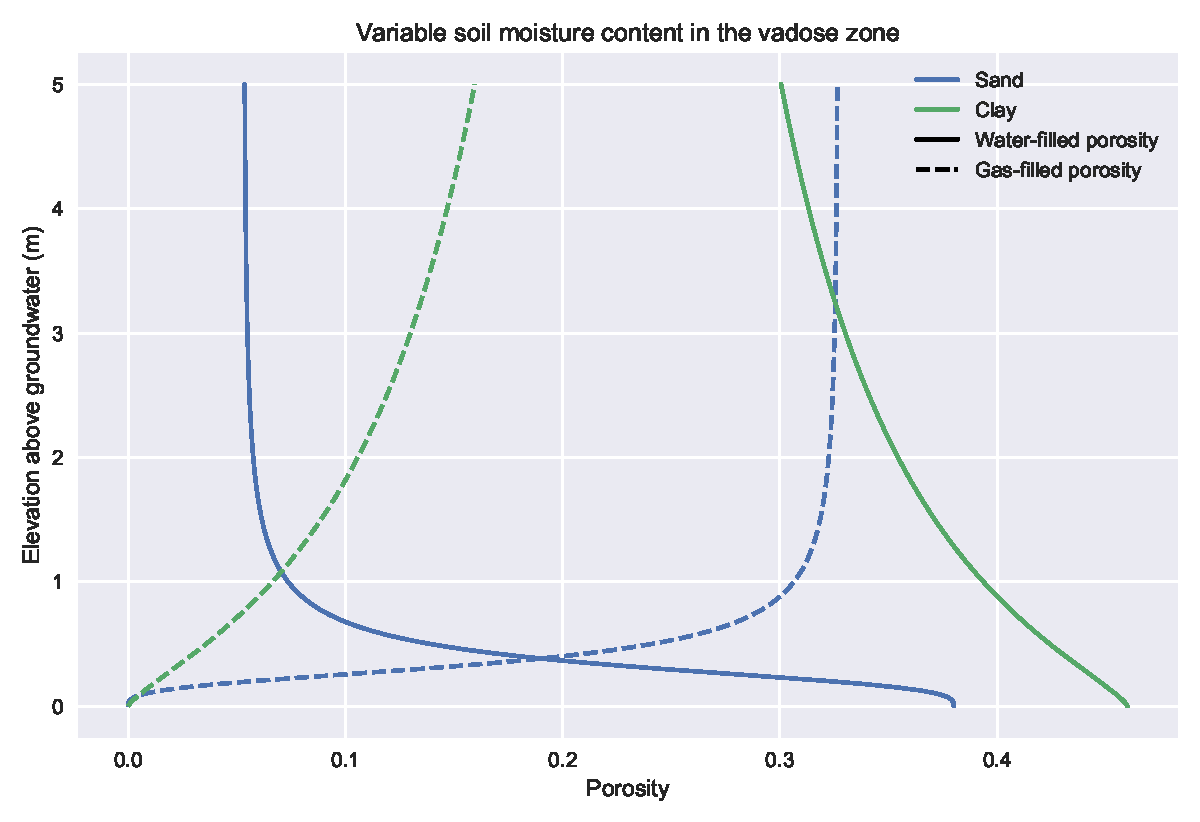
\includegraphics{van_genuchten.pdf}
  \caption{Retention curves for sandy loam soil.}
  \label{fig:van_genuchten}
\end{figure}

\subsubsection{Richard's Equation}

The change in soil moisture through a soil domain is the sum of any change in flux of water in or out of the soil domain.
In 1931 Lorenzo Richards\cite{richards_capillary_1931} developed an eponymous PDE that describes this.
Richards' equation itself is an extension of Darcy's Law, which governs fluid flow in saturated media (more on this in section \ref{sec:darcys}).
\begin{equation}\label{eq:richards}
  \rho \Big( \frac{C_m}{\rho g} + \mathrm{Se}S \Big) \frac{\partial p}{\partial t} +
  \nabla \cdot \rho \Big( -\frac{\kappa_s}{\mu} k_r (\nabla p + \rho g \nabla D)\Big) =
  Q_m
\end{equation}
Here $p$ is the capillary potential; $C_m$ is the specific moisture capacity; $\mathrm{Se}$ is the effective saturation; $S$ is the storage coefficient; $\kappa_s$ is the saturated permeability of the porous media; $\mu$ is the fluid viscosity; $k_r$ is the effective permeability; $\rho$ is the fluid density; $g$ is the acceleration of gravity; $D$ is the elevation or head; and $Q_m$ is a source term, a positive or negative value represent a source or sink respectively.\par

In the VI model that we are developing we usually assume that there is no change in soil moisture content w.r.t. time, i.e. that it is at steady-sate, and that there is no source or sink present, greatly simplifying \eqref{eq:richards}.
Since we're solving the PDE at steady-state, it is not that important to specify any initial values (although it can reduce computation time), but we need to specify a few boundary conditions to solve \eqref{eq:richards}.

\subsubsection{Boundary conditions}

In the simplest case only three boundary conditions need to be specified.
The first two are Dirichlet boundary conditions\footnote{A prescribed fixed value to the dependent value at the boundary.} where we specify the pressure to be zero at the water table boundary (bottom of the model) and at the ground surface the pressure head is equal the negative of the depth to the water table.
The third is a no-flow boundary condition\footnote{A Neumann boundary condition.}, specifying that there is no soil moisture flux through these boundaries, is applied to all other boundaries.
\begin{align}\label{eq:richards_bc}
  &\text{Water table} &p = 0 \; \mathrm{(Pa)}\\
  &\text{Ground surface} &p =  -z\rho g \; \mathrm{(Pa)} \\
  &\text{Remaining} &-\vec{n}\cdot\rho_\mathrm{water}\vec{u} = 0
\end{align}
Where $\rho$ is the density of water; $z$ is the depth of the water table relative to the ground surface; $g$ is the acceleration of gravity; $\vec{n}$ is the a boundary's normal vector; $\vec{u}$ is the velocity vector of the water moving in the soil matrix.\par
